\graphicspath{{figs/Chp-FMGaBP/}}

%%Fakesection Abstract
\glsreset{acr:fmgabp}


\chapter{Parallel Multigrid Adaptation for the Finite Element Gaussian Belief Propagation Algorithm}
\label{chp:FMGaBP}

%%Fakesection Abstract
In this chapter we introduce a novel parallel multigrid algorithm, referred to as the \gls{acr:fmgabp} algorithm, to accelerate the convergence of the previously introduced \gls{acr:fgabp} algorithm.
The \gls{acr:fmgabp} reduces the iteration count required for convergence to a competitive level while maintaining all the parallelism features of the original \gls{acr:fgabp} algorithm.
The \gls{acr:fmgabp} algorithm processes the \gls{acr:fem} computation in a fully distributed and parallel manner, with stencil-like element-by-element operations, while eliminating all global algebraic operations.
To our knowledge, this is the first multigrid formulation for continuous domain Gaussian \gls{acr:bp} type algorithms.
Similar to the \gls{acr:fgabp} algorithm, the \gls{acr:fmgabp} algorithm finds the solution to the variational formulation of the \gls{acr:fem} problem in a distributed manner.
In comparison with \gls{acr:mgpcg} solvers, the \gls{acr:fmgabp} algorithm demonstrates considerable iteration reductions as tested by Laplace benchmark problems.
In addition, the parallel implementation of the \gls{acr:fmgabp} algorithm shows a speedup of up to 2.9 times over the parallel implementation of \gls{acr:mgpcg} using eight CPU cores.


\section{Introduction}
The \gls{acr:pwgabp} algorithm, introduced by \cite{bib:Shental2008GBPSSLE,bib:Weiss01CorrectnessBelief}, was discussed in Chapters \ref{chp:PW-GaBP} and \ref{chp:relGaBP} illustrating great potential to parallelize the solving stage of the \gls{acr:fem} \cite{bib:El-Kurdi2012EIOGBPSFLSDDLS,bib:El-Kurdi2012RGBP}.
In addition, \gls{acr:pwgabp} has been shown to outperform classical iterative solvers such as \gls{acr:gs} and Jacobi \cite{bib:Shental2008GBPSSLE}.
However such algorithms, which are derived based on pairwise interconnect assumptions on the underlying \gls{acr:gm}, suffer mostly from a lack of convergence when diagonal dominance properties are not met.
In \chpRef{chp:FGaBP}, the \gls{acr:fgabp} algorithm was introduced which addresses the convergence shortcomings of \gls{acr:pwgabp} and improves the parallel efficiency of the \gls{acr:fem} computation.
While the \gls{acr:fgabp} was demonstrated to efficiently solve \gls{acr:fem} problems in parallel, element-by-element; however the \gls{acr:fgabp}'s convergence rate tends to stall when executed on fine meshes.


In this work we address this issue by introducing the novel \gls{acr:fmgabp} algorithm.
Our results for various scheduling versions of \gls{acr:fmgabp} demonstrate high convergence rates independent of the scale of discretization on the finest mesh.
In addition, we show for a benchmark Laplace problem that the \gls{acr:fmgabp} requires, in certain cases, less iterations than the \gls{acr:mgpcg} solver.
The eight thread multicore implementation of \gls{acr:fmgabp} demonstrates speedups of up to 2.9 times over the \gls{acr:mgpcg} solver based on sparse algebraic operations as implemented by the multithreaded library \libName{deal.II}~\cite{bib:dealii2007}.


The chapter is organized as follows.
In \secRef{sec:fmgabp} we present the detailed formulation of the \gls{acr:fmgabp} algorithm.
Then in \secRef{sec:fmgabpImp} we present the implementation details of the \gls{acr:fmgabp} algorithm.
Finally in \secRef{sec:FMGaBP_res} we conclude with numerical and performance results and discussions.


\section{The FMGaBP Algorithm}
\label{sec:fmgabp}

Multigrid acceleration schemes \cite{bib:Trottenberg2001M,bib:Briggs2000AMT} provide optimal convergence speeds resulting in a number of iterations almost independent of the discretization level of the \gls{acr:fem} mesh.
It is expected that the \gls{acr:fgabp} algorithm can benefit greatly from multigrid schemes mainly because, \gls{acr:bp} communications on coarser levels can serve as bridges to communications between far away nodes on finer levels.
This has the effect of considerably improving the propagation of information in the \gls{acr:femfg} model and hence speeding up the overall convergence.
In this section, we introduce an efficient adaptation of multigrid schemes to the \gls{acr:fgabp} algorithm resulting in the \gls{acr:fmgabp} algorithm.
As will be shown later, the resulting \gls{acr:fmgabp} algorithm demonstrates convergence rates independent of the \gls{acr:fem} domain's discretization level.
In addition, the \gls{acr:fmgabp} retains the distributed nature of computations, which has important implications for \gls{acr:hpc} implementations. 
Mainly, the \gls{acr:fmgabp} level transfer operations are computationally decoupled and localized without requiring any global sparse algebraic operations.


The \gls{acr:fmgabp} algorithm considerably improves the \gls{acr:fgabp} convergence rate while maintaining high parallel efficiency of stencil-like, element-by-element, operations.
Our results will later demonstrate that not only the \gls{acr:fmgabp} shows considerable advantage in parallel efficiency, but also, compared to the \gls{acr:mgpcg}, the \gls{acr:fmgabp} shows iteration reductions in certain cases.
The distinguishing feature of the \gls{acr:fgabp} algorithm is solving the \gls{acr:fem} in parallel, element-by-element, without assembling a large sparse matrix or performing any global algebraic operations such as \glspl{acr:smvm}.
This key advantage, which has important impacts on parallel hardware implementations, is maintained by the new multigrid formulation for \gls{acr:fmgabp}.


\subsection{Hierarchical Mesh Refinement}


A brief overview of multigrid schemes was presented in \secRef{sec:RMG}.
In our derivation of the \gls{acr:fmgabp} algorithm, we will be considering \gls{acr:gmg} schemes with hierarchical meshes.
In hierarchical mesh refinement schemes, local element splitting is used to generate a hierarchy of multigrid levels.
As an example, \figRef{fig:split} shows hierarchical refinement by starting from an initial coarse triangular mesh and then splitting each triangle into four geometrically similar child triangles by inserting nodes at midpoints of the parent triangle's edges.
Similar refinement can be used for quadrilateral and hexahedral meshes, where each quadrilateral (parent) is split into four child-quadrilaterals and each hexahedron (parent) is split into eight child-hexahedrons.
Each level of the hierarchy will be represented by a unique \gls{acr:femfg} graph; as will be shown later, the transfer operations will only occur between the factor nodes of the corresponding parent-child elements.
In addition, this hierarchical refinement scheme will provide key advantages for element-by-element parallel behavior of the \gls{acr:fmgabp}.
Also, by utilizing semi-irregular mesh hierarchies, more adaptation to arbitrary domains can be achieved than by using only structured meshes hierarchies.


However, and more importantly, the choice of the hierarchical refinement is not due to any imposed limitations from the \gls{acr:fmgabp} algorithm, but rather, it is used as an initial proof-of-concept phase to better illustrate the new \gls{acr:fmgabp} algorithm.
One approach to handle geometries with fine and complex features is to use non-conforming adaptive refinement \cite{bib:Becker2001AOCAAPEEFEM,bib:Bangerth2003AFEMDF} which will require special care to handle the non-conforming grid points.
In addition, adaptive refinement schemes rely on computing error estimations from a local element-by-element perspective which makes formulating the \gls{acr:fmgabp} for such refinement schemes an interesting future research direction.


\subsection{The Factor Node Belief}

To illustrate the \gls{acr:fmgabp} formulation, we start by defining a multivariate distribution, associated with each individual \fn{a}, referred to as the factor node belief $b_a(U_a)$, denoted for short as \fnb{a}.
The belief \fnb{a} function takes the form:
\begin{equation}
	b_{a}^{(t)}(U_{a}) \propto \Psi_{a}(U_{a}) \prod_{i\in\mathcal{N}(a)}\eta_{ia}^{(t)}(U_{i}), \label{eqn:genFB}
\end{equation}
where $U_a$ is the vector of random unknowns linked to \fn{a}.
In essence the belief \fnb{a}, in contrast with the nodal belief \vnb{i} as defined in \eqnRef{eqn:genB}, represents the marginal distribution as seen from \fn{a} in a particular iteration $t$.
When we use the \gls{acr:femfg} setting, the factor belief $b_a$ takes a Gaussian multivariate form as:
\begin{equation}
	b_{a}^{(t)}(U_a) \propto\exp\left[-\frac{1}{2}U_{a}^{T}W_{a}^{(t)}U_{a}+(K_{a}^{(t)})^{T}U_{a}\right] \label{eqn:gaussFB}
\end{equation}
where the parameters $W_a$ and $K_a$ represent the inverse covariance and the source vector of the factor node respectively.
Note that the function \fnb{a} takes an iterative form, where the matrix $W_a$ and the vector $K_a$ are updated each iteration according to the \gls{acr:fgabp} update rules in (\ref{eqn:fWK}).


By observing the dynamics of the message update rules of the \gls{acr:bp} algorithm in (\ref{eqn:genFNUM}), (\ref{eqn:genVNUM}), and (\ref{eqn:genB}), we can show that at message convergence the joint mean vector of \fnb{a}, given by $W_{a}^{-1}K_a$ as computed locally from the factor node's perspective, will be equal to the marginal means of $U_a$ as computed from the nodal perspective by (\ref{eqn:vnm}).
That is, if we form a vector of nodal marginal means as computed by the \gls{acr:fgabp} rule \eqnRef{eqn:vnm} in the vector $\bar{\mu}_a$ for the set of nodes connected to \fn{a}, then at message convergence we obtain:
\begin{align}
	\bar{\mu}_a & = \left[\mu_{\mathcal{L}(j)}\right],\,\,\text{where } j\in\mathcal{N}(a)\\
	& = W_{a}^{-1}K_a \label{eqn:fpMarj}
\end{align}
and $\mathcal{L(\cdot)}$ is the mapping of global variable node indices to local factor node indices.


In order to demonstrate this result, we start by formulating the marginal for $U_i$, denoted as $\tilde{b}_{i}(U_{i})$, from the defined \fnb{a} using the general \gls{acr:bp} message communication as follows:
\begin{align}
	\tilde{b}_{i}^{(t)}(U_{i})& \propto\underset{U_{\mathcal{N}(a)\setminus i}}{\int} b_{a}^{(t)}(U_{a})\ \mathrm{d}U_{\mathcal{N}(a)\setminus i}\\
	& \propto\underset{U_{\mathcal{N}(a)\setminus i}}{\int}\Psi_{a}(U_{a})\prod_{j\in\mathcal{N}(a)}\eta_{ja}^{(t)}(U_{j})\ \mathrm{d}U_{\mathcal{N}(a)\setminus i}.
\end{align}
Since at $j=i$, $\eta_{ia}(U_{i})$ is a function of the single variable node $U_i$, hence we can take it outside the integral as:
\begin{equation}
	\tilde{b}_{i}^{(t)}(U_{i}) \propto \eta_{ia}^{(t)}(U_{i})\underset{U_{\mathcal{N}(a)\setminus i}}{\int}\Psi_{a}(U_{a})\prod_{j\in\mathcal{N}(a)\setminus i}\eta_{ja}^{(t)}(U_{j})\ \mathrm{d}U_{\mathcal{N}(a)\setminus i}.
\end{equation}
Here, we are considering the case where all the \gls{acr:bp} messages are stationary, then we can substitute the \gls{acr:bp} update rules \eqnRef{eqn:genFNUM}, \eqnRef{eqn:genVNUM} and \eqnRef{eqn:genB} which results in:
\begin{align}
	\tilde{b}_{i}^{(t)}(U_{i}) & \propto\left[\prod_{k\in\mathcal{N}(i)\setminus a}m_{ki}^{(t)}(U_{i})\right]m_{ai}^{(t)}(U_{i})\\
	& \propto\prod_{k\in\mathcal{N}(i)}m_{ki}^{(t)}(U_{i})\\
	& \propto b_{i}^{(t)}(U_{i}).
\end{align}
The above result states that, at message convergence the marginal of a particular variable node computed using a factor belief function is equivalent to the marginal distribution of that node computed from the nodal perspective incorporating global information as in \eqnRef{eqn:vnm}.
Now, since for multivariate Gaussian distributions the marginal mean of a variable is equal to its corresponding value in the joint mean vector; therefore, at message convergence, the Gaussian means as computed from the local belief perspective will be in agreement with the marginal means as computed from global perspective as stated in \eqnRef{eqn:fpMarj}.

\subsection{Local Belief Residual-Correction}
Given the belief condition in \eqnRef{eqn:fpMarj}, then for each factor on a fine grid we can formulate a quantity referred to as the belief residual $r_a$ given by:
\begin{equation}
	r_a^{(t)} = K_a^{(t)} - W_a^{(t)} \bar{\mu}_a^{(t)} \label{eqn:br}.
\end{equation}
When hierarchical mesh refinement is used, the belief residuals of each group of child elements can locally be restricted into the parent element as:
\begin{equation}
	K^H_a =\mathcal{R}_l r^{h}_a \label{eqn_rr}
\end{equation}
where $K^H_a$ is the source vector of the parent element, $r^{h}_a$ is the accumulated local residual of child elements, and $\mathcal{R}_l$ is the child-parent local restriction operator.
Notice that we dropped the iteration count $(t)$ since we are operating in the same iteration for both sides of the equations.


Similarly, we can use local interpolation operations in order to apply the corrections from the coarse elements as follows:
\begin{equation}
	\bar{\mu}_a^h \gets \bar{\mu}_a^h + \mathcal{I}_l \bar{\mu}_a^H.
\end{equation}
Using the level updated $\bar{\mu}_a^h$ we can reinitialize the corresponding level local messages using again \eqnRef{eqn:br} but with $r_a \to 0$, then solving for the local factor messages as follows:
\begin{align}
	K_a^h & = W_a \bar{u}_a^h\\
	\mathcal{B}_a^h & = K_a^h - B_a^h. \label{eqn:messCorr}
\end{align}


Since we are only considering linear problems, the $\alpha$ messages are only dependent on the factor matrices which are not affected by the residual-correction multigrid scheme.
Therefore, the $\alpha$ messages retain their previous value on each level transfer.
It was found by experimentation on first order \gls{acr:fem} problems, that the $\mathcal{R}_l$ is typically the transpose of $\mathcal{I}_l$ up to a constant factor as follows:
\begin{equation}
	\mathcal{R}_l = c \left(\mathcal{I}_l\right)^T \label{eqn:galerkinCnd}
\end{equation}
where $c$ was found to equal to $1$ for structured quadrilateral and hexahedral meshes, while it was equal to $\frac{1}{3}$ for semi-irregular triangular meshes.


\subsection{Local Transfer Operations}
The \gls{acr:fmgabp} local transfer operations can be enhanced by the definition of local node numbering schemes between each set of parent-child elements.
The parent-child numbering scheme facilitates the transfer of residuals from child nodes to parent nodes using logical index computations.
As a result, the \gls{acr:fmgabp} transfer operations take the form of local stencil-like operation.
\figRef{fig:quadTrans} shows the residual transfer operations from one child node to the corresponding parent nodes using a particular local numbering scheme.
The local transfer scheme can be generalized to 3D meshes.
For example, when refining a hexahedron into eight hexahedrons, the nodes on the faces of the refined hexahedron will have weightings similar to the ones illustrated in \figRef{fig:quadTrans}, while the node in the interior will have a weighting equal to $\frac{1}{8}$.
In the case of triangular and tetrahedral meshes, the nodal weights will consist of $1$ and $\frac{1}{2}$ only.

\begin{figure}
	\centering
	{
	\subfloat[Child-a]{%
	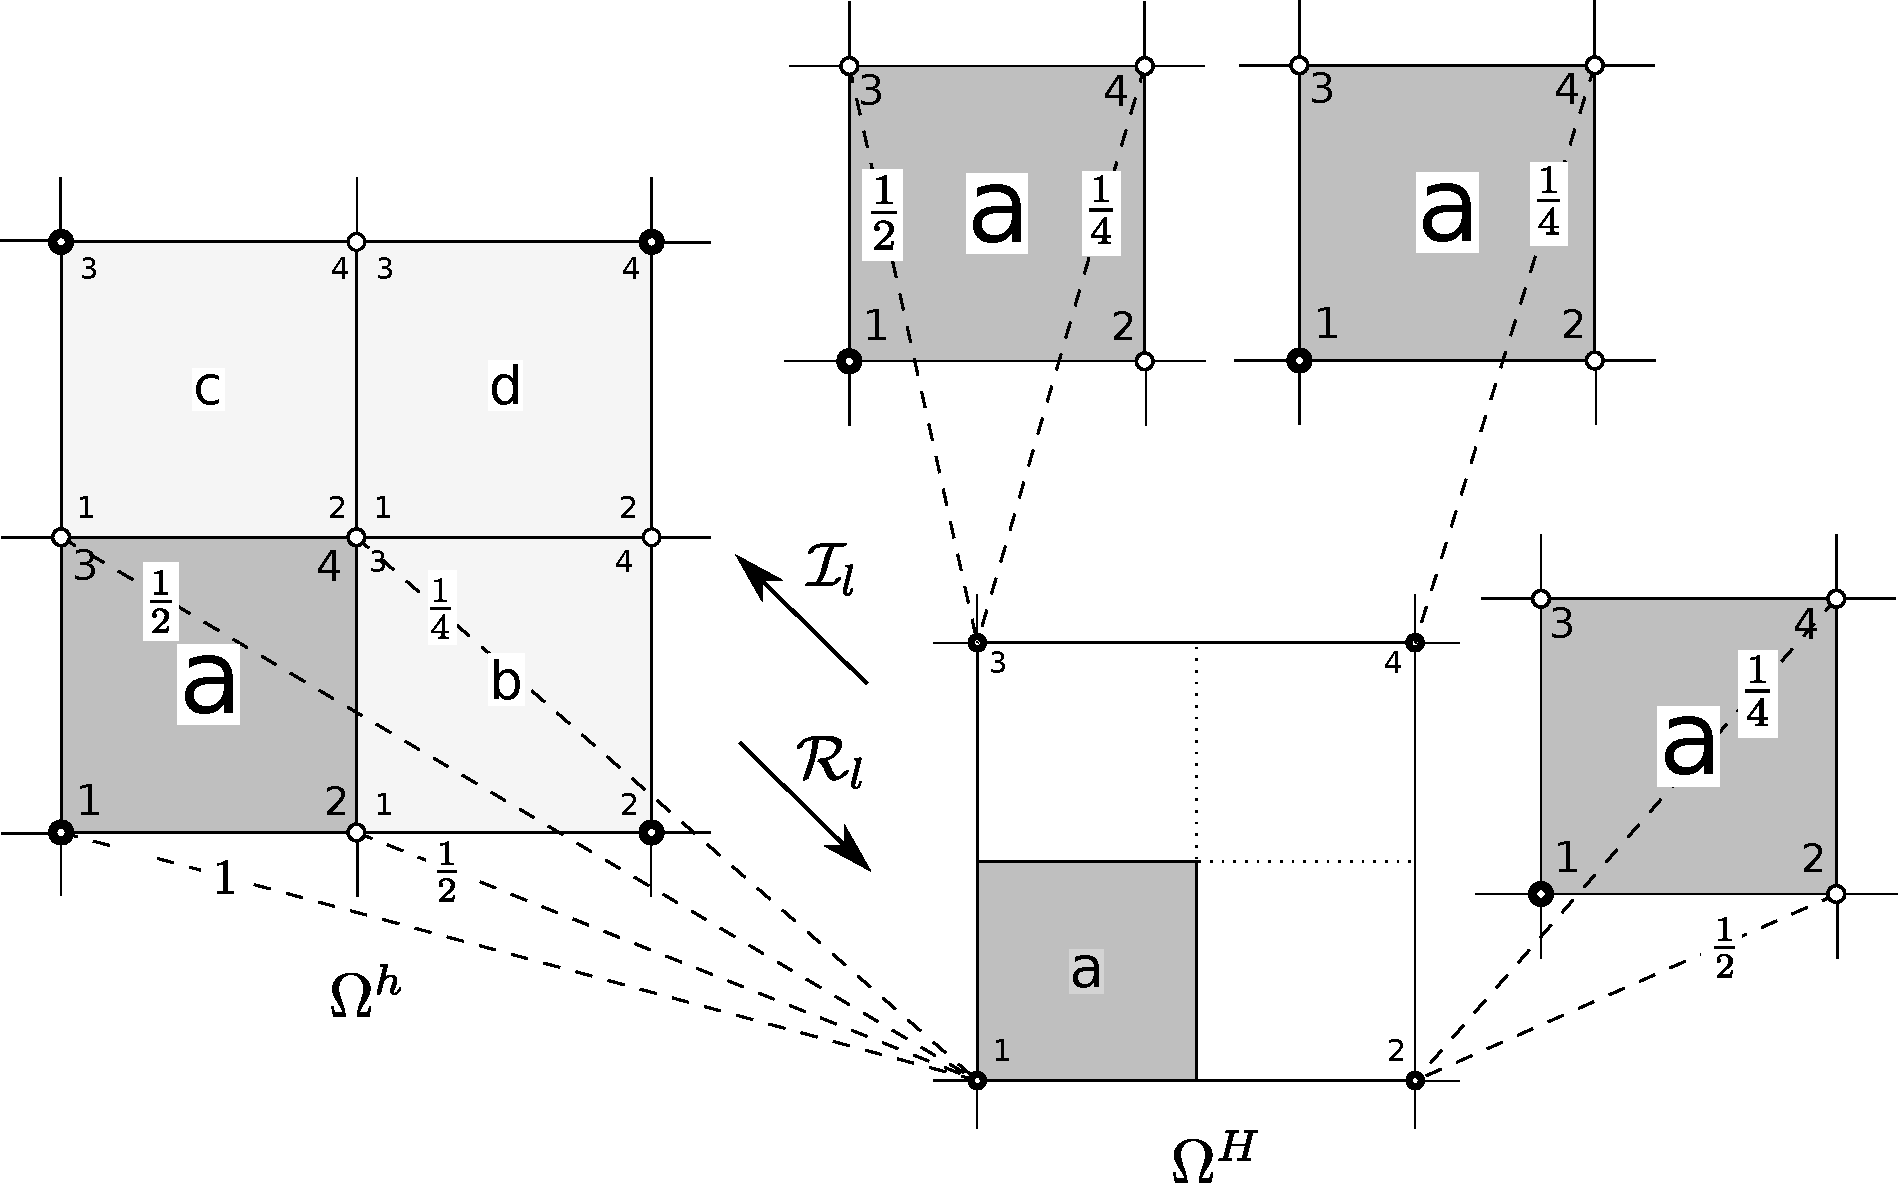
\includegraphics[scale=.4]{quad_trans_a} \label{fig:quadTrans_a}
	}
	\vfil
	\subfloat[Child-d]{%
	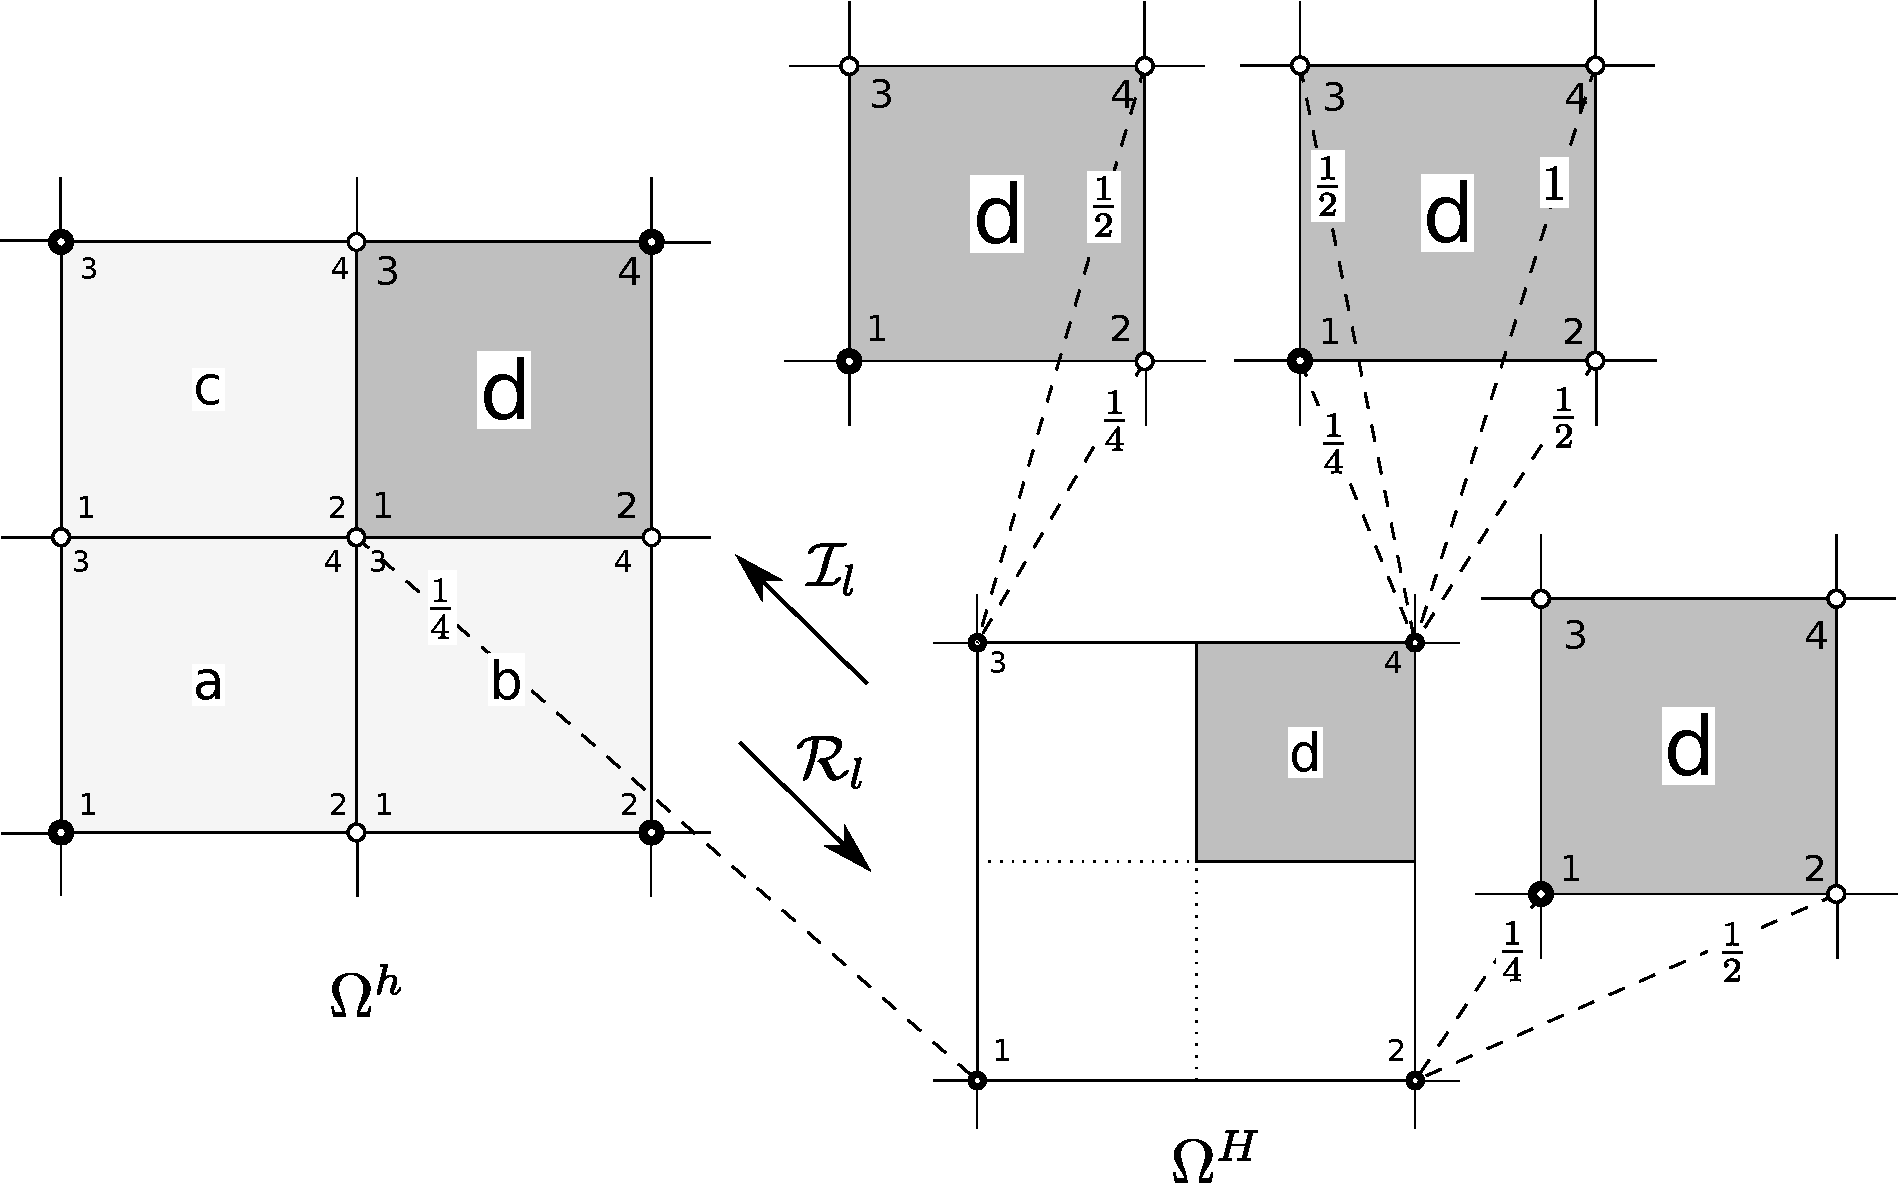
\includegraphics[scale=.4]{quad_trans_d} \label{fig:quadTrans_d}
	}
	}
	\caption[The \acrshort{acr:fmgabp} local transfer operations.]{\gls{acr:fmgabp} local transfer weights between two example child elements and the corresponding parent element. \protect\subref*{fig:quadTrans_a}~Local transfer weights for child-a. \protect\subref*{fig:quadTrans_d}~Local transfer weights for child-d.}
	\label{fig:quadTrans}
\end{figure}

Finally, It is important to note that the local \gls{acr:fmgabp} transfer operations between each set of parent-child elements create parallel operations that are also thread-safe.
This means that these local transfer operations can be implemented in an embarrassingly parallel stencil-like operations.

\subsection{The Global Residual and the Local Belief Residuals}

To illustrate the relationship between the local belief residuals and the global residual, we start by assembling a global residual vector $r_{\mathcal{G}}$ by summing all the local residual components from each factor node as follows:
\begin{equation}
	r_{\mathcal{G}} = \sum_{a \in \mathcal{S}} r_a \label{eqn:glbResSum}
\end{equation}
where $\mathcal{S}$ is the set of all factor nodes.  
Note that the sum in \eqnRef{eqn:glbResSum} is carried out by resolving mappings from local factor indices to global indices.
In the following formulas, we consider this mapping to be implicitly stated in the sum form.
Also in order to define the residual for a particular \gls{acr:bp} iteration, we assume a synchronous schedule for message communications.
This does not lead to any loss of generality, but rather it greatly simplifies the formulation since other forms of schedules may not have a clearly definable iteration.
Alternatively, one way to represent iterations is to define an iteration for every single message update.
For such a case, our formulation will also hold.

Next we substitute the local belief residual \eqnRef{eqn:br} into \eqnRef{eqn:glbResSum} to get:
\begin{align}
	r_{\mathcal{G}} & = \sum_{a \in \mathcal{S}} \left[ K_a - W_a \bar{\mu}_a \right]\\
	& = \sum_{a \in \mathcal{S}} \left[ B_a +\mathcal{B}_a - M_a \bar{\mu}_a - \mathcal{A}_a \bar{\mu}_a \right]\,\,\, \text{substituting \eqnRef{eqn:fWK}}.
\end{align}
Note that the terms $\sum_{a \in \mathcal{S}} B_a $ and $\sum_{a \in \mathcal{S}} M_a \bar{\mu}_a$ represent the assembly of the global system $f$ and $A\bar{\mu}$ correspondingly, then we have:
\begin{equation}
	r_{\mathcal{G}} = f - A\bar{\mu} + \sum_{a \in \mathcal{S}} \left[ \mathcal{B}_a -  \mathcal{A}_a \bar{\mu}_a \right] \label{eqn:glbResMess}
\end{equation}
where the dimensions of the system $A$ and $f$ are $N$, where $N$ is the total number of unknowns; and $\bar{\mu}$ is a vector of the same dimension representing the solution estimate obtained from the current \gls{acr:fgabp} level iteration.
Recall that $\mathcal{B}_a$ and $\mathcal{A}_a$ represent the factor node's incoming messages as in \eqnRef{eqn:fWK} where the incoming messages $\alpha_{ia}$ and $\beta_{ia}$ can each be substituted by \eqnRef{eqn:vna} and \eqnRef{eqn:vnb} correspondingly, then we can assemble $\mathcal{B}_a$ and $\mathcal{A}_a$ as follows:
\begin{align}
	\sum_{a \in \mathcal{S}}\mathcal{A}_a & = C \mathcal{A}_{\mathcal{G}} \label{eqn:glbA}\\
	\sum_{a \in \mathcal{S}}\mathcal{B}_a & = C \mathcal{B}_{\mathcal{G}} \label{eqn:glbB}
\end{align}
where $\mathcal{A}_{\mathcal{G}}$ is a diagonal matrix with dimension $N\text{-by-}N$ and off-diagonals equal to zero, where $N$ is the total number of unknowns; $\mathcal{B}_{\mathcal{G}}$ is a global vector of the same dimension; and $C$ is a diagonal matrix of the same dimension with constant diagonals that will be clarified shortly.
The diagonal of $\mathcal{A}_{\mathcal{G}}$ contains the nodal values $\alpha_i$ which are basically the sum of incoming $\alpha$ factor messages as in \eqnRef{eqn:vnaSum}; and similarly, the vector $\mathcal{B}_{\mathcal{G}}$ contains the sum of incoming $\beta$ factor messages as in \eqnRef{eqn:vnbSum}.
Each diagonal element of $C$ is equal to the corresponding nodes' number of links minus one.

It is easier to illustrate the assembly of $\mathcal{A}_{\mathcal{G}}$, $\mathcal{B}_{\mathcal{G}}$, and $C$ using the example diagram shown in \figRef{fig:nodalAssembly}.
If we are to assemble node index $i$ of $\mathcal{A}_{\mathcal{G}}$, then we would effectively sum all the corresponding diagonal values of $\mathcal{A}_a$, $\mathcal{A}_b$, \ldots up to $\mathcal{A}_f$, which results in:
\begin{align}
	\left[ C \mathcal{A}_{\mathcal{G}} \right]_i & = \sum_{k \in \mathcal{N}(i)} \left[ \mathcal{A}_k \right]_i\\
	& = c \alpha_i - \sum_{k \in \mathcal{N}(i)} \alpha_{ik}\\
	& = l \alpha_i - \alpha_i , \,\,\, \text{substituting \eqnRef{eqn:vnaSum}} \\
	& = (l-1) \alpha_i
\end{align}
where $l = 6$ is the number of \gls{acr:femfg} links around node $i$.
Similarly, we can perform the assembly for $\mathcal{B}_{\mathcal{G}}$.
\begin{figure}
	\centering
	{
	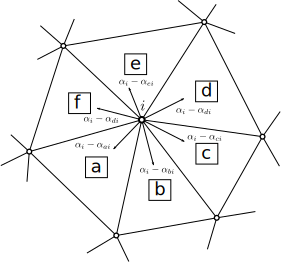
\includegraphics[scale=1.0]{glb_res}
	}
	\caption{The outgoing messages around an interior node $i$ in \acrshort{acr:femfg}.}
	\label{fig:nodalAssembly}
\end{figure}


Now substituting \eqnRef{eqn:glbA} and \eqnRef{eqn:glbB} into \eqnRef{eqn:glbResMess} we obtain:
\begin{equation}
	r_{\mathcal{G}} = f - A\bar{\mu} +  C \mathcal{B}_{\mathcal{G}} - C \mathcal{A}_{\mathcal{G}} \bar{\mu}. \label{eqn:glbResMess_2}
\end{equation}
Noting that $C \mathcal{A}_{\mathcal{G}} \bar{\mu} = C \mathcal{B}_{\mathcal{G}}$, since $[\bar{\mu}]_i = \beta_i / \alpha_i\,\,\forall i$, then \eqnRef{eqn:glbResMess_2} reduces to:
\begin{align}
	r_{\mathcal{G}} & = f - A\bar{\mu} +  C \mathcal{B}_{\mathcal{G}} - C \mathcal{B}_{\mathcal{G}}\\
	& = f - A\bar{\mu}.
\end{align}
This result illustrates that minimizing the local belief residuals is equivalent to minimizing the global residual for the assembled linear system $Au=f$, albeit computed in a distributed way without needing to assemble the sparse matrix $A$.
The result also shows that the local distributed computations performed by the \gls{acr:fmgabp} algorithm amounts to solving the same problem from global perspectives.
The reader at this point might raise the question whether it will be possible to decompose the global residual into local quantities.
In fact, such a decomposition would be hard; since without any prior knowledge of the local messages per each iteration, the decomposition would not be unique.


\subsection{The FMGaBP Fixed-Point}
Clearly from \eqnRef{eqn:br}, once all messages converge on the fine grid, that is once $\bar{\mu}_a^h \to \left[ u_0 \right]_a$ where $\left[ u_0 \right]_a$ is the true solution vector of the local nodes of $a$, then $r_a \to 0$.
Furthermore, by uniqueness of the \gls{acr:fem} solution on coarser grids, at stationarity the $\beta$ messages on each subsequent coarse grid will also be zero, hence the correction $\bar{u}_a^H$ from the coarser grids will consequently be zero.
Therefore, the \gls{acr:fmgabp} is a fixed-point algorithm for the true solution on the fine grid.

\subsection{The FMGaBP Algorithm Listing}

\algRef{alg:fmgabp} illustrates a high-level listing of the \gls{acr:fmgabp} algorithm.
The \gls{acr:fmgabp} algorithm can be seen as executing instances of the \gls{acr:fgabp} algorithm on each level in the multigrid hierarchy.
The loops on lines \ref{alg:fmgabpDownV} and \ref{alg:fmgabpUpV} traverse all the levels on the V-cycle except the coarsest level, first going down the cycle and then up the cycle.
Each level visited, the \gls{acr:fgabp} executes $v_1$ iterations down the cycle and $v_2$ iterations up the cycle.
It was found that $v_1 = v_2 =1$ is typically sufficient in most cases.
We iterate on the coarsest level using the \gls{acr:fgabp} algorithm, that is in contrast to conventional multigrid methods where a direct solver is used on the coarsest level.
Since the coarsest level contains a very small number of factors, within the order of few hundreds, its execution can be quite fast.
Also as can be noted on Line \ref{alg:fmgabpCrs}, there was no need to use a low tolerance on the coarsest level.
In many cases also, a tolerance of $10^{-6}$ was found to be sufficient on the coarsest level.
One important note to make is that the \gls{acr:fmgabp} algorithm can solve the problem down to machine floating-point precision, as can be noted by the low tolerance for convergence on Line \ref{alg:fmgabpTestTol}.

\begin{algorithm}[t]
  %\centering
	\begin{algorithmic}[1]
		\STATE Obtain \gls{acr:fem} hierarchical mesh
		\LOOP[For each level in the mesh hierarchy]
		\STATE Perform partition-color
		\STATE Generate element matrices $M_s$ and source vectors $B_s$ 
		\STATE Incorporate boundary conditions 
		\STATE \textit{Initialize:} $\alpha_{ij} = 1,\,\, \beta_{ij} = 0,\,\,\forall i,j$
		\AlgENDLOOP
		\REPEAT[\gls{acr:fmgabp} V-cycle iteration: $t=1,2,\cdots$]
		\LOOP[Traverse levels down the V-cycle] \label{alg:fmgabpDownV}
		\IF{Coarsest level reached}
		\STATE Exit
	\ENDIF
	\STATE Execute $v_1$ iterations of \gls{acr:fgabp} (\algRef{alg:FGaBP})
	\STATE Restrict residuals from child-factors into parent-factors
	\AlgENDLOOP
	\STATE Execute \gls{acr:fgabp} on coarsest level for tolerance  $<10^{-9}$ \label{alg:fmgabpCrs}
	\LOOP[Traverse levels up the V-cycle] \label{alg:fmgabpUpV}
	\STATE Prolongate corrections from parent-factors into child-factors
	\STATE Execute $v_2$ iterations of \gls{acr:fgabp} (\algRef{alg:FGaBP})
	\AlgENDLOOP
	\UNTIL{Convergence check on finest level messages for tolerance  $<10^{-16}$} \label{alg:fmgabpTestTol}
	\STATE \textit{Output:} $\mu_i = \frac{\beta_i}{\alpha_i}$
\end{algorithmic}
\caption{The \acrshort{acr:fmgabp} algorithm.}
\label{alg:fmgabp}
\end{algorithm}

\section{Implementation}
\label{sec:fmgabpImp}

\subsection{Data-Structures}

The \gls{acr:fmgabp} data-structures are mostly based on the \gls{acr:fgabp} data-structures with the addition of another dense matrix per multigrid level.
The added matrix stores the index associations of parent-child \glspl{acr:fn} for each hierarchical pair of coarse-fine levels.
The total size of the \gls{acr:fmgabp} data-structure can be obtained by:
\begin{align}
	\mathrm{FMGaBP\, Memory} & \approx O\left[ (Z+cN_f) \sum_{l=0}^{L-1} \frac{1}{c^l} - cN_f \right]\\
	& = O\left[(Z+cN_f) \frac{1-(1/c)^{L}}{1-(1/c)} - cN_f\right]
	\label{eqn:fmgabpMem}
\end{align}
where $l$ is the level index; $L$ is the total number of levels; $Z=2 \gls{acr:nv}+\gls{acr:nf}(n^2+4n)$ which is the \gls{acr:fgabp} memory on the finest level as detailed in \secRef{sec:fgabpDS}; and $c$ is the number of children, e.g. $c=4$ for 2D quadrilateral meshes or $c=8$ for 3D hexahedral meshes.
Clearly, the overall memory complexity is linear in \gls{acr:nv} as $L\to \infty$.

\subsection{Multicore CPU Implementation}

Similar to the \gls{acr:fgabp}, the \gls{acr:fmgabp} code was designed using C++ \gls{acr:oop} \cite{bib:c++stroustrup2013,bib:c++prata2004}.
This facilities the integration of the \gls{acr:fgabp} code as a level solver into the \gls{acr:fmgabp} with minimal recoding.
In addition, different \gls{acr:fem} open-source libraries, such as \dealName{} \cite{bib:dealii2007} and \libName{GetFEM++} \cite{bib:getfem}, can be integrated easily which enables thorough testing of the \gls{acr:fmgabp} algorithm.
The library \libName{GetFEM++} was used to test our code using irregular triangular meshes that are generated by \libName{Gmsh} \cite{bib:gmsh2009}, while \dealName{} was used to test our code on quadrilateral and hexahedral meshes.
However out of the two, only \dealName{} provides parallel implementation of its solver and therefore it will be used for our performance analysis.
While there are other high quality C++ \gls{acr:fem} libraries such as \libName{Dune} \cite{bib:dunefemwebpage,bib:dunefemwebpage} and \libName{libMesh} \cite{bib:libMesh}, \dealName{} and \libName{GetFEM++} were the most up-to-date with extensive documentation and active support teams.


Another advantage of using \gls{acr:oop} style coding is that the \gls{acr:fmgabp} implementation performance can be tested using different \gls{acr:blas} libraries and dense solvers \cite{bib:blas,bib:blasDongarra:2002,bib:lapack}.
These libraries are needed by the \glspl{acr:fn} for the efficient execution of its dense operations, such as the Cholesky inversion or the \gls{acr:gs} iteration required by the \gls{acr:aufgabp} scheme.
For that purpose, we used different dense routines from the libraries \dealName{}, \libName{gmm} \cite{bib:gmm}, and \libName{Eigen} \cite{bib:eigen}.
\libName{Eigen}, however, seemed to produce the best overall results.


Similar to the \gls{acr:fgabp} code, the \gls{acr:fmgabp} code was parallelized using \libName{OpenMP} \cite{bib:openmp}.
Each thread is assigned to handle the transfer operations of each parent-child \glspl{acr:fn} set.
The transfer operations are fully decoupled; and hence, there was no need for the use of elaborate partitioning schemes such as coloring in order to ensure thread-safety.
A single thread synchronization directive is used at the end of each transfer operation either restriction or prolongation.
Finally, the output solution was visualized using \libName{Paraview} \cite{bib:paraview}.



\subsection{Manycore GPU Implementation}

In the past decade, architectures with many (tens or hundreds of) integrated cores have been introduced and used in the scientific computing community.
\Glspl{acr:gpu} are a popular class of manycore processors offering greater opportunities of parallelism on a single chip than multicore CPUs.
It is expected that adeptly parallel algorithms such as the \gls{acr:fmgabp} can benefit from the increased parallelism of \gls{acr:gpu} architectures.
In this section, we will detail the implementation techniques used to evaluate the \gls{acr:fmgabp} performance on \gls{acr:gpu} architectures.

\subsubsection{Background on GPUs}

Attempts to port parts or all of the \gls{acr:fem} computations to manycore architectures have been presented in previous works.
Most of these works are aimed at accelerating either the global sparse matrix assembly or the global system solve stage.
Constrained by the special characteristics of their applications, the works in \cite{bib:Bolz2003SMSGPUs,bib:rodriguez2006NSM} present simple assembly strategies suited for manycore architectures.
Their proposed techniques are not applicable for general \gls{acr:fem} applications but, rather, are mostly suited to the sparsity structure of their specific applications.
Graph coloring schemes in \cite{bib:Komatitsch2009PHF,bib:Hesthaven2007NDG,bib:Cris2011assemblyGPU} are used to partition the \gls{acr:fem} elements to non-overlapping sets, in order to enable a parallel thread-safe execution of the assembly routines for the global sparse matrix.
Assembling a global sparse matrix, to be solved in a separate stage, based on graph coloring and partitioning can be costly.
For the \gls{acr:fgabp} algorithm, coloring adds little overhead since the global sparse matrix is never assembled and coloring is used, rather, to compute the \gls{acr:fem} solution in parallel.
Other work \cite{bib:Dziekonski2013generation,bib:Dziekonski2012finite,bib:Fu2014architecting} propose strategies and novel sparse storage formats to reduce the memory footprint of the assembled sparse matrix.
Since, \gls{acr:fgabp} eliminates the need for assembling a large sparse matrix, many of the optimizations proposed in previous work are, thus, not applicable to our work.

Significant research has been aimed at improving the solve stage for sparse systems using \glspl{acr:gpu}.
Most these works focus on accelerating the execution of the compute intensive kernels in the Krylov solvers.
As shown in \cite{bib:Hoemmen2010EECS,bib:Mehridehnavi2013CAGPU} such efforts are mainly communication bound and are limited by the maximum performance achieved from parallelizing the compute intensive kernels.
The assembled matrix is usually large and sparse and in many cases does not fit in the small and fast access memory levels of CPU and the co-processor memory.


\gls{acr:fgabp} avoids assembling a global sparse matrix and, thus, is a promising candidate for manycore architectures.
Instead of solving a large sparse matrix, each \gls{acr:fgabp} iteration needs to compute the incoming and outgoing messages for each factor node.
The compute intensive kernel in a \gls{acr:fgabp} iteration involves computing the inverses of many small dense matrices; an operation that is embarrassingly parallel and well suited for manycore architectures.
Coloring the \gls{acr:femfg} models improves the underlying parallelism significantly and allows \glspl{acr:fn} of the same color to be processed in parallel by hundreds of threads without causing any synchronization or memory collisions when accessing the \gls{acr:vn} data.
To demonstrate the embarrassingly parallel nature of both the \gls{acr:fgabp} and \gls{acr:fmgabp} algorthims, we have implemented them on the {NVIDIA} Tesla {C2075} \gls{acr:gpu}.


\subsubsection{The GPU architecture}

The {NVIDIA} Tesla {C2075} \gls{acr:gpu}, which belongs to the Fermi generation, is used to illustrate the performance of the \gls{acr:fmgabp} implementation on manycore architectures.
The Tesla {C2075} has a 6~\gls{acr:gb} {DRAM} memory, 448 {CUDA} cores, 48~\gls{acr:kb} of shared memory, and a memory bandwidth of 144~\gls{acr:gbps}.

Current {NVIDIA} \glspl{acr:gpu} consist of \glspl{acr:sm} each containing a few \glspl{acr:sp}, an on-chip shared memory, a data cache and a register file.
Threads executing on each \gls{acr:sm} have access to the same shared memory and register file, which enables communication and data synchronization with little overhead.
Threads executing on different \glspl{acr:sm} can only synchronize through the \glspl{acr:gpu} off-chip global \gls{acr:dram} which incurs high latency of several hundred clock cycles.
To parallelize an algorithm on \glspl{acr:gpu}, all of these architectural features have to be taken into account to efficiently use the available \gls{acr:gpu} resources.

The most popular \glspl{acr:api} used to implement algorithms on \glspl{acr:gpu} are the \gls{acr:cuda} and the \gls{acr:opencl}.
\gls{acr:cuda} 5.0 was used along with the library \libName{CUBLAS} 5.0 \cite{bib:Nvi11b} to implement the \gls{acr:fmgabp} algorithm on the \gls{acr:gpu}.
Initially, data has to be explicitly transferred from the CPU memory to \gls{acr:gpu} followed by the instantiation of a collection of kernels executing the parallel segments of the program on the \gls{acr:gpu}.
Threads are grouped into blocks that are scheduled for execution on the \gls{acr:gpu}'s \gls{acr:sm}.
Groups of 32 threads in a block, called warps, are scheduled to execute the same instruction at the same time.
Threads in the same block can communicate via on-chip shared memory with little latency while threads in different blocks have to go through the \gls{acr:gpu} global memory for any kind of data synchronization \cite{bib:Nvi11b}.


\subsubsection{GPU implementation details}
The \gls{acr:fmgabp} algorithm is fully implemented on the {NVIDIA} Tesla {C2075}.
The \glspl{acr:fn}, \glspl{acr:vn}, and level matrix data are transferred to the \gls{acr:gpu} once, thus no GPU-CPU memory transfers are required during the algorithm's execution.
The following details the \gls{acr:gpu} implementation of the \gls{acr:fmgabp} algorithm:


\textbf{\textsl{Multigrid restriction and prolongation kernels:}} The restriction and prolongation stages are implemented in two different kernels.
The parent-child mappings in the \gls{acr:fmgabp} are loaded into shared memory to reduce global memory references.
The compute intensive operation in the multigrid computations is the dense matrix vector multiply for each parent \gls{acr:fn} in the coarser grid.
The number of parent \glspl{acr:fn} assigned to each warp is computed by dividing the number of threads per warp (32) by the number of children for each parent.
For example, in a 2D problem using quadrilateral meshes, each warp in the interpolation kernel applies corrections from eight \glspl{acr:fn} in the coarse grid to their children; thus allocating four threads to each \gls{acr:fn} in the coarse grid to parallelize the compute intensive kernels involved in the restrict operations.


\textbf{\textsl{Batch of inverses on GPUs:}} Computing the inverse of local matrices in the smoother iterations is the most time consuming operation in the \gls{acr:fmgabp} algorithm.
Depending on the problem size, the number of matrices to be inverted can be very large.
Various heuristics could be used to compute a batch of inverses on the \gls{acr:gpu}.
Depending on the size of the local matrices, each inverse could be computed via one thread block, one warp or even one thread.
For example, if the rank of each matrix is 256 then allocating one thread block (with 256 threads) to each matrix inverse would be efficient. 


A batch of inverses can be computed using the {NVIDIA}'s {CUBLAS} library \cite{bib:Nvi11b} for matrices up to rank 32.
An in-place LU decomposition should first be performed and then the \libName{cublasDgetriBatched} kernel is called to compute an out-of-place batch inversion.
Since each warp computes the inverse of one matrix, the aforementioned kernel does not perform well for the low rank matrices in the \gls{acr:fmgabp} kernel.
For 2D problems using quadrilateral meshes or 3D problems using tetrahedral meshes, our matrices are only of rank 4, thus when using the \libName{CUBLAS} matrix inversion, the \gls{acr:gpu} resource will be underutilized and threads in a warp will not have enough work.
Our matrix inversion kernel is customized to the matrix's dimension.
The number of inverses computed via one warp is obtained through dividing the number of threads per warp (32) by the rank of the local dense matrices.
For example, for a 2D problem with rank 4 local matrices, each warp computes 8 matrix inversions.
We outperform the \libName{CUBLAS} matrix inversion kernel by 2$\times$ when inverting a batch of 10 million rank 4 matrices.
Another major advantage of our matrix inverse kernel is that it performs the inverse in-place on shared memory.
As a result, the computed inverses do not have to be stored in global memory and the outgoing messages can be computed in the same kernel.
Not storing the matrix inverses in the global memory enables the \gls{acr:gpu} to solve larger problems more readily.


\textbf{\textsl{Kernel fusion in FGaBP:}} The \gls{acr:fgabp} iterations involve computing the incoming and outgoing messages and updating the \gls{acr:vn}'s running sums.
Instead of calling three separate \gls{acr:gpu} kernels one for each stage, we fuse these kernels and only call one \gls{acr:gpu} kernel for each iteration.
Key advantages resulting from the fusion process are:
First, data can be loaded into shared memory in order to be used by a single \gls{acr:fgabp} kernel call reducing communication within the \gls{acr:gpu}'s memory hierarchy.
Second, the local matrix inverses can be generated on the fly and used to compute the running sum without the need to be stored in global memory.
Lastly, kernel call overheads are also reduced by only calling one kernel for each \gls{acr:fgabp} iteration.


\section{The FMGaBP Numerical Results and Discussions}
\label{sec:FMGaBP_res}

The performance of the \gls{acr:fmgabp} algorithm is demonstrated using two Laplace benchmark problems as shown in \figRef{fig:ps}.
The first problem is the \gls{acr:ssc} using two different material properties as shown in \figRef{fig:msf}.
The second problem is the \gls{acr:lsc} as shown in \figRef{fig:lsf}.
Both problems employ Dirichlet and Neumann boundary conditions.


The \gls{acr:ssc} problem was formulated using the library \libName{GetFEM++} \cite{bib:getfem} with semi-irregular triangular meshes.
The \gls{acr:lsc} problem was formulated using the library \libName{deal.II} \cite{bib:dealii2007} with hierarchical quadrilateral meshes.
Since the library \libName{deal.II} inherently supports hierarchical meshes and multigrid solvers using parallel implementations, it was used for performance comparisons.
A V-cycle multigrid scheme is used in all our experiments.
All solvers are terminated when the residual $l^2$-norm is dropped to $10^{-15}$.
The \gls{acr:fmgabp} algorithm uses the iterative \gls{acr:fgabp} as the coarsest level solver; whereas, a Householder direct solver was used by \libName{deal.II} on the coarse level for the \gls{acr:mgpcg} solver.


\subsection{Semi-irregular Mesh Hierarchy}

\tableRef{tbl:sscItr} shows the \gls{acr:fmgabp} convergence results for the \gls{acr:ssc} problem.
The results demonstrate a convergence performance almost independent of the number of unknowns in the finest level.
However, a trend of slightly increasing number of iterations is observed.
This increase is expected as a result of the strongly varying material coefficients (20:1) as shown in \figRef{fig:msf}.

%1-coarse & 825   & 1556  & --- \tabularnewline
\begin{table}
	\centering
	\begin{threeparttable}[c]
		\caption[The \acrshort{acr:fmgabp} algorithm performance for the \acrshort{acr:ssc} problem.]{The \acrshort{acr:fmgabp} algorithm performance for the \acrshort{acr:ssc} problem using five levels of refinement.} \label{tbl:sscItr}
  %\renewcommand{\tabcolsep}{.1cm}
		\begin{tabular}{crr>{\itshape}c} \toprule
			Refinement & Unknowns & Triangles & Iterations           \tabularnewline
			Level      &          &           & $v_{1}=1,\, v_{2}=1$ \tnote{*} \tabularnewline
			\midrule
			1-coarse   & 222      & 382       & ---  \tabularnewline
			2          & 825      & 1,528     & 9    \tabularnewline
			3          & 3,177    & 6,112     & 11   \tabularnewline
			4          & 12,465   & 24,448    & 13   \tabularnewline
			5          & 49,377   & 97,792    & 15   \tabularnewline
			6          & 196,545  & 391,168   & 16   \tabularnewline
			\bottomrule
		\end{tabular}
		\begin{tablenotes}
			\begin{footnotesize}
			\item[*] {The parameters $v_{1}$ and $v_{2}$ are pre and post V-cycle iterations.}
			\end{footnotesize}
		\end{tablenotes}
	\end{threeparttable}
\end{table}


\subsection{Structured Mesh Hierarchy}

\tableRef{tbl:lscItr} shows the \gls{acr:fmgabp} results for the \gls{acr:lsc} problem compared with the results from \libName{deal.II}.
The basic \gls{acr:fgabp} algorithm was used as the level solver for the \gls{acr:fmgabp} algorithm.
The library \libName{deal.II} implements the \gls{acr:mgpcg} solver using multithreading.
The symbols $t_{st}$ and $t_{sv}$ refer to the setup and solve time respectively reported in seconds; the acronym ``itr'' refers to iterations.
The timing results were obtained using a compute node from the supercomputing cluster Colesse \cite{bib:colesse}.
The computing node contains two quadcore Xeon Nehalem CPUs @ 2.8 GHz with 8 \gls{acr:mb} cache and 48~\gls{acr:gb} \gls{acr:dram}.
Problem sizes up to to 12.6 million unknowns are solved.
A coloring algorithm is used to guarantee thread safety.
The coloring algorithm required minimal overhead, by virtue of utilizing the hierarchical structure of the mesh provided by \libName{deal.II}.
For all timing cases, the best of forty runs is reported.

\begin{table}
	\centering
	\begin{threeparttable}[c]
		\caption[The \acrshort{acr:fmgabp} speedup over \libName{deal.II} on a 2D domain.]{The \acrshort{acr:fmgabp} speedup over \libName{deal.II} on a 2D domain using 8-threads on $2\times$quadcore processors.} \label{tbl:lscItr}
	%\renewcommand{\arraystretch}{1.05}
		\begin{tabular}{llllllll>{\itshape}r>{\itshape}r} \toprule
			\multirow{2}{22mm}{Unknowns (million)} & \multirow{2}{27mm}{Quadrilaterals (million)} & \multicolumn{3}{c}{\gls{acr:fmgabp}} & \multicolumn{3}{c}{\gls{acr:mgpcg}} & \multicolumn{2}{c}{\textit{Speedup}}\tabularnewline
	  %\cline{3-5}
			\cmidrule(r){3-5} \cmidrule(r){6-8}\cmidrule(r){9-10}
			&       & itr & $t_{st} $ & $t_{sv}$ & itr & $t_{st}$ & $t_{sv}$ & setup & solve\tabularnewline
			\midrule
			0.788    & 0.786 & 6             & 2.6                & 0.98               & 10  & 6.14     & 2.56     & 2.4   & 2.6 \tabularnewline
			3.15     & 3.15  & 6             & 10.5               & 3.74               & 10  & 27.5     & 10.4     & 2.6   & 2.8 \tabularnewline
			12.6     & 12.6  & 6             & 43.1               & 14.2               & 10  & 108      & 41.6     & 2.5   & 2.9 \tabularnewline
			\bottomrule
		\end{tabular}
	\end{threeparttable}
\end{table}

As shown in \tableRef{tbl:lscItr}, the \gls{acr:fmgabp} algorithm required a considerably lower number of iterations than the \gls{acr:mgpcg} solver on this particular problem.
In addition, the \gls{acr:fmgabp} algorithm demonstrates considerable time speedups for both the setup time and the solve time.
Since setup operations are not parallelized in \libName{deal.II} at the time of using the library, sequential execution time is only reported for the setup phase.
The major reductions in setup time was due to the fact that the \gls{acr:fmgabp}, unlike to the library \libName{deal.II}, does not require the setup of globally large sparse matrices, or level transfer matrices.
The \gls{acr:fmgabp} algorithm also demonstrated parallel solve time speedups of up to 2.9 times over \libName{deal.II}'s \gls{acr:mgpcg} solver.
The speedups were due to mainly two factors, the considerable iteration reductions and the higher parallel efficiency of \gls{acr:fmgabp}.
As a key factor, the \gls{acr:fmgabp} implements the level transfer operations using embarrassingly parallel local stencil-like operations.


\tableRef{tbl:fmgabpHelm3D} shows the \gls{acr:fmgabp} results for the Helmhotlz problem on a 3D domain as introduced in \secRef{sec:fgabpVer}.
The \gls{acr:aufgabp} algorithm was used as the level solver for the \gls{acr:fmgabp} algorithm configured with 2 \gls{acr:gs} iterations and $10^{-1}$ tolerance for the $\alpha$ messages.
The \gls{acr:fmgabp} is compared with the \gls{acr:mgpcg} solver implemented with multithreading by \libName{deal.II}.
The similarity in the iteration counts between the two solvers is simply coincidental.
The timing results were obtained using a compute node from the supercomputing cluster Sandybride on SciNet \cite{bib:scinet}.
The node contains 2$\times$8-core Xeon CPUs @ 2.5 GHz with 8~\gls{acr:mb} cache and 64~\gls{acr:gb} \gls{acr:dram}.
Problem sizes up to 16.97 million unknowns are solved.
A coloring algorithm is used to guarantee thread safety.
For all timing cases, the best of forty runs is reported.

The \gls{acr:fmgabp} algorithm demonstrated similar timing speedups over the multithreaded implementation of \gls{acr:mgpcg} by the library \libName{deal.II}. 
These speedups are attributable to the \gls{acr:fmgabp}'s efficient utilization of parallel CPU's resources.
While the library \libName{deal.II} requires the buildup of globally shared sparse-data structures for each multigrid level, the \gls{acr:fmgabp} algorithm uses dense data-structures.
This also explains the speedups obtained by the setup time which can be considered high compared to the solve time.


\begin{table}[t]
	\centering
	\begin{threeparttable}[c]
		\caption[The \acrshort{acr:fmgabp} speedup over \libName{deal.II} on a 3D domain.]{The \acrshort{acr:fmgabp} speedup over \libName{deal.II} on a 3D domain using 24-threads on $2\times$6-core processors.} \label{tbl:fmgabpHelm3D}
	%\renewcommand{\arraystretch}{1.05}
		\begin{tabular}{llllllll>{\itshape}r>{\itshape}r} \toprule
			\multirow{2}{22mm}{Unknowns (million)} & \multirow{2}{27mm}{Quadrilaterals (million)} & \multicolumn{3}{c}{\gls{acr:fmgabp}} & \multicolumn{3}{c}{\gls{acr:mgpcg}} & \multicolumn{2}{c}{\textit{Speedup}}\tabularnewline
	  %\cline{3-5}
			\cmidrule(r){3-5} \cmidrule(r){6-8}\cmidrule(r){9-10}
			         &       & itr & $t_{st} $ & $t_{sv}  $ & itr & $t_{st}$      & $t_{sv}$ & setup & solve\tabularnewline
			\midrule
			0.036 & 0.033 & 8 & 0.54 & 0.15 & 8            & 0.90 & 0.17 & 1.67 & 1.13 \tabularnewline
			0.275 & 0.262 & 8 & 3.19 & 0.78 & 8            & 7.48 & 1.51 & 2.34 & 1.94 \tabularnewline
			2.147 & 2.097 & 8 & 25.0 & 5.56 & 8            & 62.2 & 11.5 & 2.5  & 2.07 \tabularnewline
			16.97 & 16.78 & 8 & 212. & 52.9 & -- \tnote{*} & --   & --   & --   & --   \tabularnewline
			\bottomrule
		\end{tabular}
		\begin{tablenotes}
			\begin{footnotesize}
			\item[*] {\libName{deal.II} crashed for the experiment with 16.97 million unknowns.}
			\end{footnotesize}
		\end{tablenotes}
	\end{threeparttable}
\end{table}


\figRef{fig:psu} shows the speedup factors of \gls{acr:fmgabp} for the different problem sizes on 2D and 3D domains.
\gls{acr:fmgabp} demonstrates approximately linear trends of speedups with increasing number of threads.
In addition, the graph trends show increased parallel efficiency as the problem size increases.

\begin{figure}
	\centering{
	\subfloat[]{
	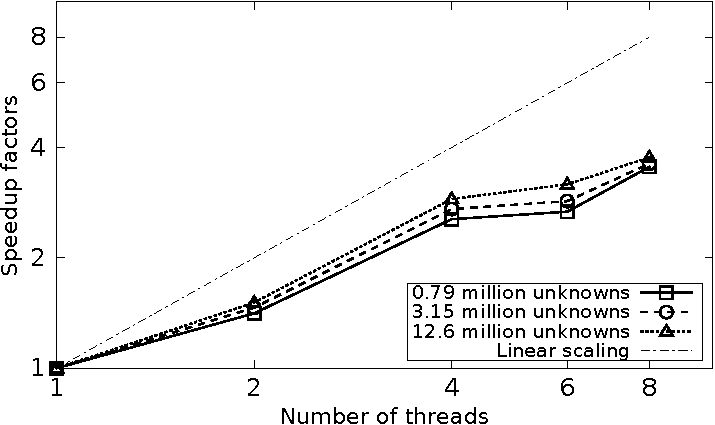
\includegraphics[scale=1.0]{psu} \label{fig:psu_2d}
	}
	\vfill
  %\hspace{+1mm}
	\subfloat[]{
	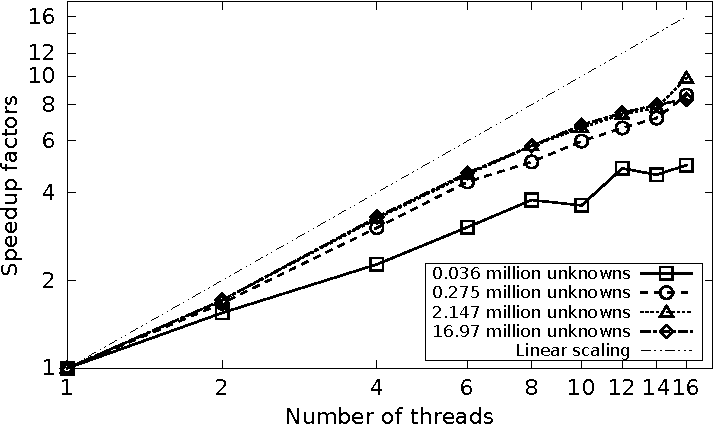
\includegraphics[scale=1.0]{psu_3d} \label{fig:psu_3d}
	}
	}
	\caption[The \acrshort{acr:fmgabp} speedup factors for the 2D and 3D problems.]{\protect\subref*{fig:psu_2d}~The \acrshort{acr:fmgabp} speedup factors for the 2D \gls{acr:ssc} problem on $2\times$quadcore processors node. \protect\subref*{fig:psu_3d}~The \acrshort{acr:fmgabp} speedup factors for the 3D Helmholtz problem on $2\times$8-core processors node.}
	\label{fig:psu}
\end{figure}



To address problems of larger scale, the use of multi-node clusters is required.
For such implementations, the \gls{acr:mpi} programming model is typically used along with sophisticated partitioning algorithms.
Implementations of \gls{acr:fmgabp} using \gls{acr:mpi} are proposed as a future research direction.


\subsection{Manycore GPU Performance}

The \gls{acr:fmgabp} is implemented on an {NVIDIA} Tesla {C2075} for the 2D Helmhotlz problem, as previously defined in \secRef{sec:fgabpVer}, with the number of unknowns ranging from 26K to 4.1M.
Larger problems should be executed on a cluster of \glspl{acr:gpu} because of the \gls{acr:gpu}'s global memory size limits. 
\figRef{fig:gpuRes} shows the speedup achieved by implementing \gls{acr:fmgabp} on a single \gls{acr:gpu} versus the proposed parallel CPU implementation of the method on the SciNet Sandybride cluster node \cite{bib:scinet}.
The SciNet node contains 2$\times$8-core Xeon 2.0~GHz CPUs with 64~\gls{acr:gb} \gls{acr:dram}.
The speedup scalability is also presented in the figure by altering the number of threads for the CPU runs. 
As shown in the figure, the Tesla C2075 outperforms the CPU with up to 12 cores for all problem sizes. 
Larger problems are able to utilize the GPU resources more efficiently thus the GPU is faster than the 16-core CPU node for the largest problem with 4.1M unknowns.
The only case where the GPU did not demonstrate speedups were for the smaller problem sizes (26K and 1M unknowns). 
The average (speedup over all problem sizes) achieved from the GPU implementation compared to the dual-core, quad-core and 12-core CPU settings are 4.8$\times$, 2.3$\times$ and 1.5$\times$ respectively.

\begin{figure}[t]
	\centering{
	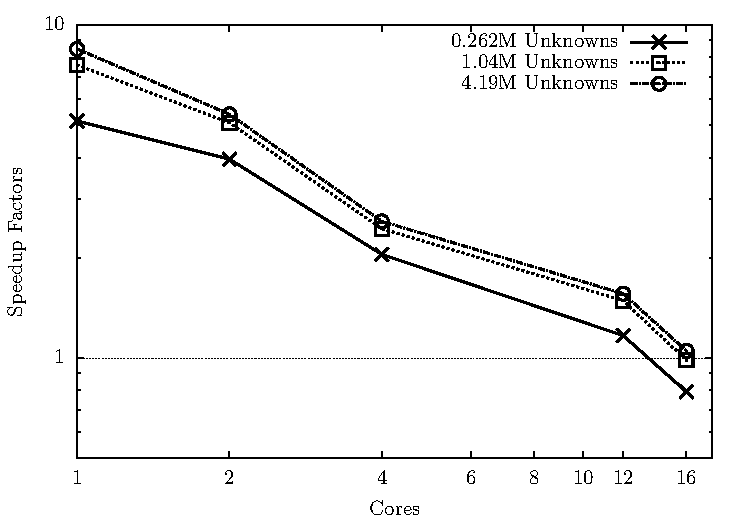
\includegraphics[scale=1.0]{plot_gpu_su.pdf}
	}
	\caption[The FMGaBP GPU implementation speedups.]{The speedup achieved from accelerating FMGaBP on NVIDIA Tesla C2075 compared to the parallel implementation of the method on 1-16 CPU cores.}
	\label{fig:gpuRes}
\end{figure}

\section{Conclusion}
The novel \gls{acr:fmgabp} algorithm was introduced and was shown to achieve high parallel performance due to its matrix-free approach and localized computations.
In addition, we showed for a benchmark Laplace problem that the \gls{acr:fmgabp} algorithm requires less iterations than the \gls{acr:mgpcg} solver.
The threaded multicore implementation of \gls{acr:fmgabp} demonstrates speedups of up to 2.9$\times$ over \libName{deal.II}'s implementation of \gls{acr:mgpcg}.
The GPU implementation showed considerable speedups over the multithreaded CPU implementation.





